\section{Solve \kSUM using only \SmallO{n}-linear queries}


\begin{figure}
\centering
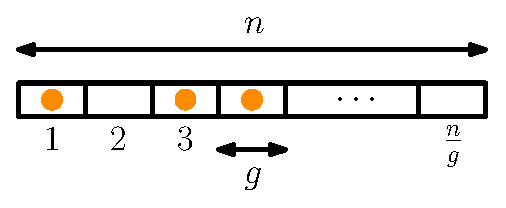
\includegraphics[width=0.4\textwidth]{fig/point-location/blocks}
\caption{Solving the problem for blocks \(1\), \(3\) and \(4\) only.}
\label{fig:point-location:on:blocks}
\end{figure}

We have seen that using Meiser's algorithm, one can solve the \kSUM problem
with \BigO{n^3 \log^3 n} queries.

We have also seen that the queries the algorithm is required to make can
involve up to \(n\) linear terms and are thus \(n\)-linear.

We show that it is possible to restrict ourselves to \SmallO{n}-linear queries
with the addition of a factor \(n\) to the complexity of the algorithm.

Now look at \ref{fig:point-location:on:blocks}. We represent input set \(\S\)
using a vector \(\enum{x_1,\ldots,x_n}\) of size \(n\). The trick is the
following. Instead of using Meiser's algorithm once to solve the problem of
size \(n\), we will divide the input vector in blocks of size \(g\) and solve a
\kSUM problem for all comvinations of \(k\) blocks.  There are \(\sfrac{n}{g}\)
such blocks hence the number of problems to solve is \(\binom{\sfrac{n}{g}}{k}
= \BigO{(\frac{n}{g})^k} \).

The complexity of solving all the problems would then be
\begin{displaymath}
\BigO{\group{\frac{n}{g}}^k (kg)^3 \log^3 (kg) }
\end{displaymath}
and the queries are \((kg)\)-linear.

By choosing \(g = n^{\frac{k-1}{k}} = n^{1-\frac{1}{k}}\) and we obtain a
complexity of
\begin{displaymath}
\BigO{n (kn^{1-\frac{1}{k}})^3 \log^3 (kn^{1-\frac{1}{k}}) }
\end{displaymath}
with \((kn^{1-\frac{1}{k}})\)-linear queries.


